\documentclass[11pt,a4paper]{article}

\usepackage[margin=2.5cm]{geometry}
\usepackage[T1]{fontenc}
\usepackage[utf8]{inputenc}
\usepackage{amsmath}
\usepackage{booktabs}
\usepackage{array}
\usepackage{graphicx}
\usepackage{subcaption}
\usepackage{hyperref}
\usepackage{xcolor}
\usepackage{parskip}

\hypersetup{
    colorlinks=true,
    linkcolor=blue,
    urlcolor=blue,
    citecolor=blue
}

\graphicspath{
    {build/comparison/}
    {build/pycsep/}
    {build/pycsep_1d/}
    {../build/comparison/}
    {../build/pycsep/}
    {../build/pycsep_1d/}
}

\newcommand{\Mc}{M_c}

\title{Issue-Time Sensitivity of Operational ETAS Forecasts for the\\
2016 $M_w$ 7.8 Kaik\={o}ura Sequence}
\author{NZ ETAS Pipeline}
\date{\today}

\begin{document}
\maketitle

\begin{abstract}
We evaluate issue-time sensitivity of NZ operational ETAS forecasts for the
2016 $M_w$ 7.8 Kaik\={o}ura sequence using a fixed-horizon design in which all
eight forecasts verify the same post-mainshock window (days 7--14,
$N_{\mathrm{obs}}=323$, $M\geq\Mc=3.0$), while only the amount of early
post-mainshock data used for MLE fitting varies: a generic-parameter run plus
sequence-specific fits at 2~h, 6~h, 12~h, 1~d, 2~d, 3~d, and 7~d.
Each run contains 1000 stochastic catalogs and is evaluated with pyCSEP
catalog-based tests against a common GeoNet observed catalog.
The analysis reveals \textbf{three distinct failure regimes} whose separation
is only possible under a fixed verification horizon.
(1)~\emph{STAI and branching-identifiability failure} (generic and 2~h--1~d):
the MLE converges to a near-zero-cascade local minimum (indirect triggering
2--9\%; correct value $\approx33\%$); simulation medians are 45--103 events
(observed: 323; ratios 0.14--0.32); all N-tests fail by severe underprediction.
Critically, the analytical expectation $E[N]$ diverges enormously from the
simulation median for these runs---up to a factor of 20 for the 12~h and 1~d
windows---signalling near-supercritical ETAS dynamics in the tail of the
branching distribution.
(2)~\emph{Omori decay failure} (2~d--3~d): the MLE correctly identifies the
cascading regime (indirect triggering $\approx31\%$) but fits $p=0.90$ instead
of the true $p=1.10$, causing days 7--14 to be systematically overpredicted
(medians 492--499, ratios 1.52--1.55; N-tests fail by overprediction).
(3)~\emph{Calibrated} (7~d only): median 334 versus observed 323 (ratio 1.03),
N-test passes comfortably, and rolling Kolmogorov--Smirnov $p=0.98$.
Across all eight experiments, resampled magnitude tests and marginal
log-likelihood tests pass universally, confirming that the Gutenberg--Richter
magnitude distribution is well-captured regardless of issue time.
Spatial support remains incomplete in all runs (16--25 observed events in
zero-rate cells), indicating a persistent kernel-support limitation orthogonal
to the count-calibration question.
We propose two distinct identifiability barriers---a branching barrier crossed
near 2~d and an Omori barrier crossed near 7~d---and argue that Bayesian
hierarchical priors on the Omori $p$-value would be the highest-leverage
improvement for the 2~d--3~d regime.
\end{abstract}

\textbf{Keywords}: ETAS; operational aftershock forecasting; pyCSEP;
Kaik\={o}ura; catalog incompleteness; New Zealand.

\section{Introduction}

Operational aftershock forecasting is fundamentally an issue-time problem: the
question is not only whether a model is good, but whether it becomes useful
quickly enough after a large mainshock to support decisions in the first hours
to days. Modern operational systems therefore do not wait a week before issuing
aftershock forecasts. USGS OAF begins automatic updates within minutes and then
reissues through the first hours and days \cite{usgs_schedule,usgs_overview}.
The official USGS background documentation makes clear that this operational
workflow spans both Reasenberg--Jones and ETAS-style public forecasts
\cite{usgs_background}.
Prospective CSEP experiments have similarly emphasized short-horizon,
rolling forecasts rather than a single retrospective fit \cite{zhuang2011,
csep_etas}.
Italy's operational earthquake forecasting program follows the same repeated
issuance logic rather than a single delayed fit
\cite{marzocchi2014,spassiani2023}.

The main obstacle to early ETAS forecasting is not lack of model flexibility but
short-term aftershock incompleteness (STAI). In the first hours to days after a
large earthquake, detection thresholds are elevated and many small events are
temporarily missing from routine catalogs
\cite{ogata2006,omi2013,omi2014,page2016,seif2017,lippiello2019,hainzl2024}.
Magnitude-of-completeness estimation therefore becomes part of the forecast
problem itself \cite{woessner2005}, and even magnitude-frequency estimation can
be biased unless transient incompleteness is handled explicitly
\cite{vandere1st2021}.
That affects ETAS productivity, Omori decay, branching, and uncertainty.
Kaik\={o}ura is a strong test case because it was both highly productive and
operationally important, and because the real-time forecast literature already
documents difficulties with the early sequence \cite{rhoades2017,harte2019}.

The goal of this manuscript is to characterize, using a completed fixed-horizon
experiment set, precisely \emph{how} and \emph{why} ETAS forecast skill changes
as the amount of early post-mainshock data increases from hours to days. The
fixed-horizon design---all eight forecasts verifying the same days 7--14
window---is now implemented and allows clean, controlled comparisons across
issue times. Our analysis shows that issue-time effects do not degrade
monotonically but instead produce three qualitatively distinct regimes, each
with a different mechanistic explanation. Recognizing these regimes clarifies
what improvements are most needed and where the leverage is greatest.

\section{Experiment Set}

\subsection{Fixed-horizon design}

This manuscript analyzes the completed run set archived in
\texttt{nz\_etas\_simulations*.txt} and the corresponding
\texttt{build/pycsep*} directories generated on 31~March--1~April 2026. Those
outputs define the experiment actually evaluated here and should be treated as
the authoritative record for this manuscript.

The archive contains one generic-parameter ETAS run and seven sequence-specific
ETAS runs at increasing issue times:
\[
0.5~\mathrm{d\ generic\text{-}conditioned},\ 2~\mathrm{h},\ 6~\mathrm{h},\
12~\mathrm{h},\ 1~\mathrm{d},\ 2~\mathrm{d},\ 3~\mathrm{d},\ 7~\mathrm{d}.
\]
The defining feature of the design is that \emph{every} run verifies the same
7-day forecast window (days 7.0--14.0 post-mainshock) against the same GeoNet
observed catalog ($N_{\mathrm{obs}}=323$, $M\geq3.0$, NZ testing region).
Because the verification target never changes, differences in pyCSEP test
outcomes are attributable solely to changes in the fitting data window, not
to differences in the forecast horizon or observation period.

Each run produces 1000 stochastic simulations with $\Mc=3.0$,
$M_{\mathrm{max}}=9.5$, and a maximum of 10 ETAS generations.
The early issue-time branch (2~h, 6~h, 12~h, 1~d) uses
\texttt{timeDependentMc = true} to mitigate catalog incompleteness during
fitting; the 2~d, 3~d, and 7~d runs use \texttt{timeDependentMc = false},
consistent with the expectation that catalog completeness is largely recovered
within two days for this sequence.

\subsection{Design decisions}

Three aspects of the design deserve explicit statement.
First, the \emph{generic} run is not a strict time-zero baseline: it is
initialized with the first 0.5~d aftershock list and then uses NZ generic
prior parameters without sequence-specific MLE fitting. It is therefore a
\emph{generic-parameter conditioned} forecast, which provides a meaningful
no-fit reference but is not strictly equivalent to a pre-mainshock prior.
Second, the \texttt{timeDependentMc} branch choice is a scientifically
motivated design decision that is itself part of the experiment: as shown in
Section~\ref{sec:mag_freq}, it is necessary but not sufficient to resolve early
forecast skill.
Third, any comparison of count results between issue times is clean only under
the fixed-horizon design; the reader should not compare these results to any
earlier version of this experiment that used varying verification windows.

\subsection{Experiment design table}

\begin{table}[ht]
\centering
\small
\caption{Fixed-horizon experiment design. All runs verify the same forecast
window (days 7.0--14.0 post-mainshock, $N_{\mathrm{obs}}=323$). The
\texttt{tdMc} column indicates whether \texttt{timeDependentMc=true} was used
during MLE fitting.}
\label{tab:design}
\begin{tabular}{llllll}
\toprule
Run & Data window & Forecast window & Duration & \texttt{tdMc} & Model \\
\midrule
Generic prior (no MLE) & 0.0--0.5 d & 7.0--14.0 d & 7.0 d & -- & Generic parameter ETAS \\
2 h & 0.0--0.083 d & 7.0--14.0 d & 7.0 d & yes & Sequence-specific ETAS \\
6 h & 0.0--0.25 d & 7.0--14.0 d & 7.0 d & yes & Sequence-specific ETAS \\
12 h & 0.0--0.5 d & 7.0--14.0 d & 7.0 d & yes & Sequence-specific ETAS \\
1 d & 0.0--1.0 d & 7.0--14.0 d & 7.0 d & yes & Sequence-specific ETAS \\
2 d & 0.0--2.0 d & 7.0--14.0 d & 7.0 d & no & Sequence-specific ETAS \\
3 d & 0.0--3.0 d & 7.0--14.0 d & 7.0 d & no & Sequence-specific ETAS \\
7 d & 0.0--7.0 d & 7.0--14.0 d & 7.0 d & no & Sequence-specific ETAS \\
\bottomrule
\end{tabular}
\end{table}

\section{Methods}

\subsection{ETAS implementation}

The ETAS implementation uses New Zealand generic prior parameters with
$\bar{a}=-2.423$, $\bar{p}=1.08$, $\bar{c}=0.01$~d, $\alpha=1$, $b=1$, and
$M_{\mathrm{ref}}=4.5$. Sequence-specific runs perform MLE over
$a_{ms}$, $a$, $p$, and $c$ using the issue-time-specific aftershock list.
The model class is the standard Ogata ETAS family in which each event can
generate offspring that contribute to the future cascade \cite{ogata1988}.
All runs produce 1000 stochastic catalogs with a maximum of 10 generations and
$M_{\max}=9.5$.

The fixed-horizon design means that each run's MLE is computed over a different
amount of data, but every resulting parameter set is then used to generate
simulations evaluated against the same observed catalog. This makes N-test and
rolling calibration results directly comparable across all eight issue times.

The \texttt{timeDependentMc} setting is enabled for the 2~h--1~d branch,
causing the MLE to down-weight catalog intervals where detection is estimated
to be incomplete. While this is necessary to prevent STAI from biasing the
parameter estimates, it does not guarantee parameter convergence: the key
question---addressed in Section~\ref{sec:params}---is whether the available
data are sufficient to identify the branching and decay structure of the
sequence, not merely to mitigate missing events.

\subsection{pyCSEP evaluation}

We evaluate each forecast using pyCSEP catalog-based tests against a GeoNet
observed catalog matched to the forecast time window and the NZ CSEP testing
region \cite{pycsep_eval,pycsep_catalog_tutorial}. The primary metrics used in
this manuscript are:

\begin{itemize}
    \item the catalog number test (N-test), which compares $N_{\mathrm{obs}}$
          against the distribution of simulated catalog counts and returns the
          lower-tail quantile $\delta_1$ and upper-tail quantile $\delta_2$;
    \item the catalog magnitude test (M-test), which compares the
          observed magnitude--frequency distribution to the simulated ensemble;
    \item a resampled M-test, which controls for count differences by
          subsampling each simulated catalog to the observed count before
          comparing magnitude distributions;
    \item the marginal log-likelihood (MLL) test;
    \item the catalog spatial test (S-test) and pseudolikelihood test (PL-test),
          interpreted here as support diagnostics given frequent
          \texttt{status=undersampled} reports;
    \item rolling number consistency (rolling KS test $p$-value), which
          assesses whether the temporal allocation of events within the
          7--14~d window is calibrated.
\end{itemize}

\section{Results}

\subsection{Parameter evolution and identifiability regimes}
\label{sec:params}

With the fixed-horizon design, fitted parameter sets separate into three
qualitatively distinct groups (Table~\ref{tab:params}).

\begin{table}[ht]
\centering
\small
\caption{MLE parameters and indirect triggering fraction for each run.}
\label{tab:params}
\begin{tabular}{lrrrrl}
\toprule
Run & $a_{ms}$ & $a$ & $p$ & $c$ (d) & Indirect \% \\
\midrule
Generic (no MLE) & $-2.54$ & $-2.54$ & $1.08$ & $0.0079$ & $8.1\%$ \\
2 h (\texttt{tdMc}) & $-2.25$ & $-3.05$ & $1.00$ & $0.0013$ & $3.7\%$ \\
6 h (\texttt{tdMc}) & $-2.00$ & $-3.20$ & $1.00$ & $0.0021$ & $2.3\%$ \\
12 h (\texttt{tdMc}) & $-1.75$ & $-3.05$ & $0.90$ & $0.0006$ & $2.6\%$ \\
1 d (\texttt{tdMc}) & $-1.75$ & $-3.05$ & $0.90$ & $0.0006$ & $3.9\%$ \\
2 d & $-2.75$ & $-2.00$ & $0.90$ & $0.1000$ & $30.6\%$ \\
3 d & $-2.75$ & $-2.00$ & $0.90$ & $0.1000$ & $30.9\%$ \\
7 d (reference) & $-3.00$ & $-2.00$ & $1.10$ & $0.1000$ & $32.6\%$ \\
\bottomrule
\end{tabular}
\end{table}

The generic run sits near the NZ prior mean. The 2~h--1~d fits converge to a
\emph{low-cascade local minimum}: $a$ is strongly negative ($-3.05$ to
$-3.20$), $c$ is very small (0.0006--0.0021~d), and the indirect triggering
fraction is only 2.3--3.9\%, compared to 32.6\% in the converged 7~d fit.
This is not a gradual evolution but a discrete MLE failure mode: with only
hours of data, the likelihood surface is dominated by the mainshock's direct
contribution, and the MLE locks into a solution where cascading is
near-zero.

A \textbf{grid resolution artifact} is apparent at 12~h and 1~d, which produce
identical fitted parameters ($a_{ms}=-1.75$, $a=-3.05$, $p=0.90$,
$c=0.0006$~d) despite the additional 12 hours of data. This is consistent
with the finite resolution of the $21\times21\times16\times16$ MLE grid:
the two data windows are insufficiently different to move the grid optimum,
confirming that any apparent distinction between the 12~h and 1~d forecasts
is not parameter-driven.

The transition between 1~d and 2~d marks a qualitative regime shift. At 2~d the
MLE \emph{escapes} the low-cascade minimum: $a$ rises to $-2.00$, $c$ jumps to
0.1~d, and indirect triggering reaches 30.6\%---comparable to the 7~d value.
This \textbf{branching barrier} (crossed between 1~d and 2~d) represents the
minimum data window needed for the MLE to identify that aftershock-to-aftershock
cascading is a significant component of sequence productivity.

However, 2~d and 3~d data are still insufficient to identify the Omori decay
exponent accurately. Both fits return $p=0.90$, while the 7~d fit gives
$p=1.10$. Since $p$ controls the long-term tail of the Omori law, a fit with
$p=0.90$ generates too many events at days 7--14 relative to the true decay
rate. This \textbf{Omori barrier} is only fully crossed with 7~d of data.

These two barriers are conceptually distinct and require different amounts of
information. The branching barrier depends primarily on observing enough
aftershock-to-aftershock pairs to lift the $a$-value estimate; the Omori
barrier depends on observing the temporal curvature of the decay rate over a
sufficiently long baseline. Recognizing them as separate constraints is a novel
finding of this fixed-horizon experiment.

\subsection{Fixed-horizon count skill and the three failure regimes}
\label{sec:count}

Under the fixed-horizon design, all eight runs are evaluated against the same
$N_{\mathrm{obs}}=323$, making the N-test directly comparable.
Table~\ref{tab:counts} summarizes the count results and pyCSEP test outcomes.

\begin{table}[ht]
\centering
\small
\caption{Count and primary pyCSEP test results, fixed-horizon runs
(days 7--14, $M\geq3$, $N_{\mathrm{obs}}=323$).
$E[N]$ is the analytical expected count from the summary file.
Median is the pyCSEP representative-catalog count.
$(\delta_1,\delta_2)$ are the N-test lower- and upper-tail quantiles.
Resamp-M is the resampled M-test lower-tail quantile.
MLL is the marginal log-likelihood test lower-tail quantile.}
\label{tab:counts}
\begin{tabular}{lrrrrcccc}
\toprule
Run & Median & $E[N]$ & Ratio & $(\delta_1,\delta_2)$ & M-test & Resamp-M & MLL & S-test \\
\midrule
Generic & 103 & 144.9 & 0.32 & (0.003, 0.997) & (0.999, 0.001) & (0.852, 0.148) & (0.360, 0.640) & (0.014, 0.986) \\
2 h & 54 & 252.6 & 0.17 & (0.000, 1.000) & (1.000, 0.000) & (0.805, 0.195) & (0.369, 0.631) & (0.000, 1.000) \\
6 h & 50 & 432.2 & 0.15 & (0.000, 1.000) & (1.000, 0.000) & (0.824, 0.176) & (0.376, 0.624) & (0.000, 1.000) \\
12 h & 45 & 921.3 & 0.14 & (0.000, 1.000) & (1.000, 0.000) & (0.744, 0.256) & (0.390, 0.610) & (0.000, 1.000) \\
1 d & 51 & 928.7 & 0.16 & (0.000, 1.000) & (1.000, 0.000) & (0.847, 0.153) & (0.377, 0.623) & (0.000, 1.000) \\
2 d & 499 & 403.5 & 1.55 & (0.998, 0.002) & (0.297, 0.703) & (0.832, 0.168) & (0.340, 0.660) & (0.941, 0.059) \\
3 d & 492 & 417.5 & 1.52 & (0.992, 0.008) & (0.302, 0.698) & (0.840, 0.160) & (0.324, 0.676) & (0.956, 0.044) \\
7 d & 334 & 265.7 & 1.03 & (0.594, 0.411) & (0.736, 0.264) & (0.821, 0.179) & (0.356, 0.644) & (0.963, 0.037) \\
\bottomrule
\end{tabular}
\vspace{4pt}
\raggedright
\footnotesize
Ratio = Median/$N_{\mathrm{obs}}$. PL-test upper-tail quantiles (from Table~\ref{tab:support})
are 0.011 (Generic), 0.000 (2~h--1~d), 0.018 (2~d), 0.016 (3~d), 0.031 (7~d).
\end{table}

\vspace{6pt}
\noindent\textbf{Regime 1 (Generic and 2~h--1~d): STAI and branching-identifiability failure.}
Simulation medians range from 45 to 103 events, giving median-to-observed ratios
of 0.14--0.32. Every N-test in this regime has $\delta_2=1.000$: all 1000
simulations predict fewer events than the 323 observed, a complete failure by
underprediction. This failure is not simply a consequence of catalog
incompleteness---\texttt{timeDependentMc=true} is enabled for the 2~h--1~d
runs---but reflects a deeper identifiability failure: the MLE solution has zero
(or near-zero) cascading, so each simulation is driven almost entirely by the
mainshock's direct triggering. The resulting catalogs are systematically
deficient.

\vspace{6pt}
\noindent\textbf{Regime 2 (2~d--3~d): Omori decay failure.}
After the branching barrier is crossed, the regime reverses sharply.
Simulation medians of 499 and 492 far exceed $N_{\mathrm{obs}}=323$
(ratios 1.55 and 1.52). N-tests now fail by overprediction:
$\delta_1=0.998$ at 2~d and $\delta_1=0.992$ at 3~d, meaning nearly all
simulations predict more events than observed. The branching regime is
correctly identified, but the too-shallow Omori exponent ($p=0.90$ instead of
1.10) generates an artificially elevated rate at days 7--14.

\vspace{6pt}
\noindent\textbf{Regime 3 (7~d): Calibrated.}
The 7~d fit produces a median of 334 against $N_{\mathrm{obs}}=323$, a ratio
of 1.03. The N-test passes comfortably with $(\delta_1,\delta_2)=(0.594,0.411)$,
indicating that the observed count is well within the central body of the
simulated distribution. Both the branching structure and the Omori decay rate
are now correctly identified. The PL-test and S-test remain undersampled (see
Section~\ref{sec:spatial}), but the count and temporal calibration are sound.

\begin{figure}[ht]
\centering
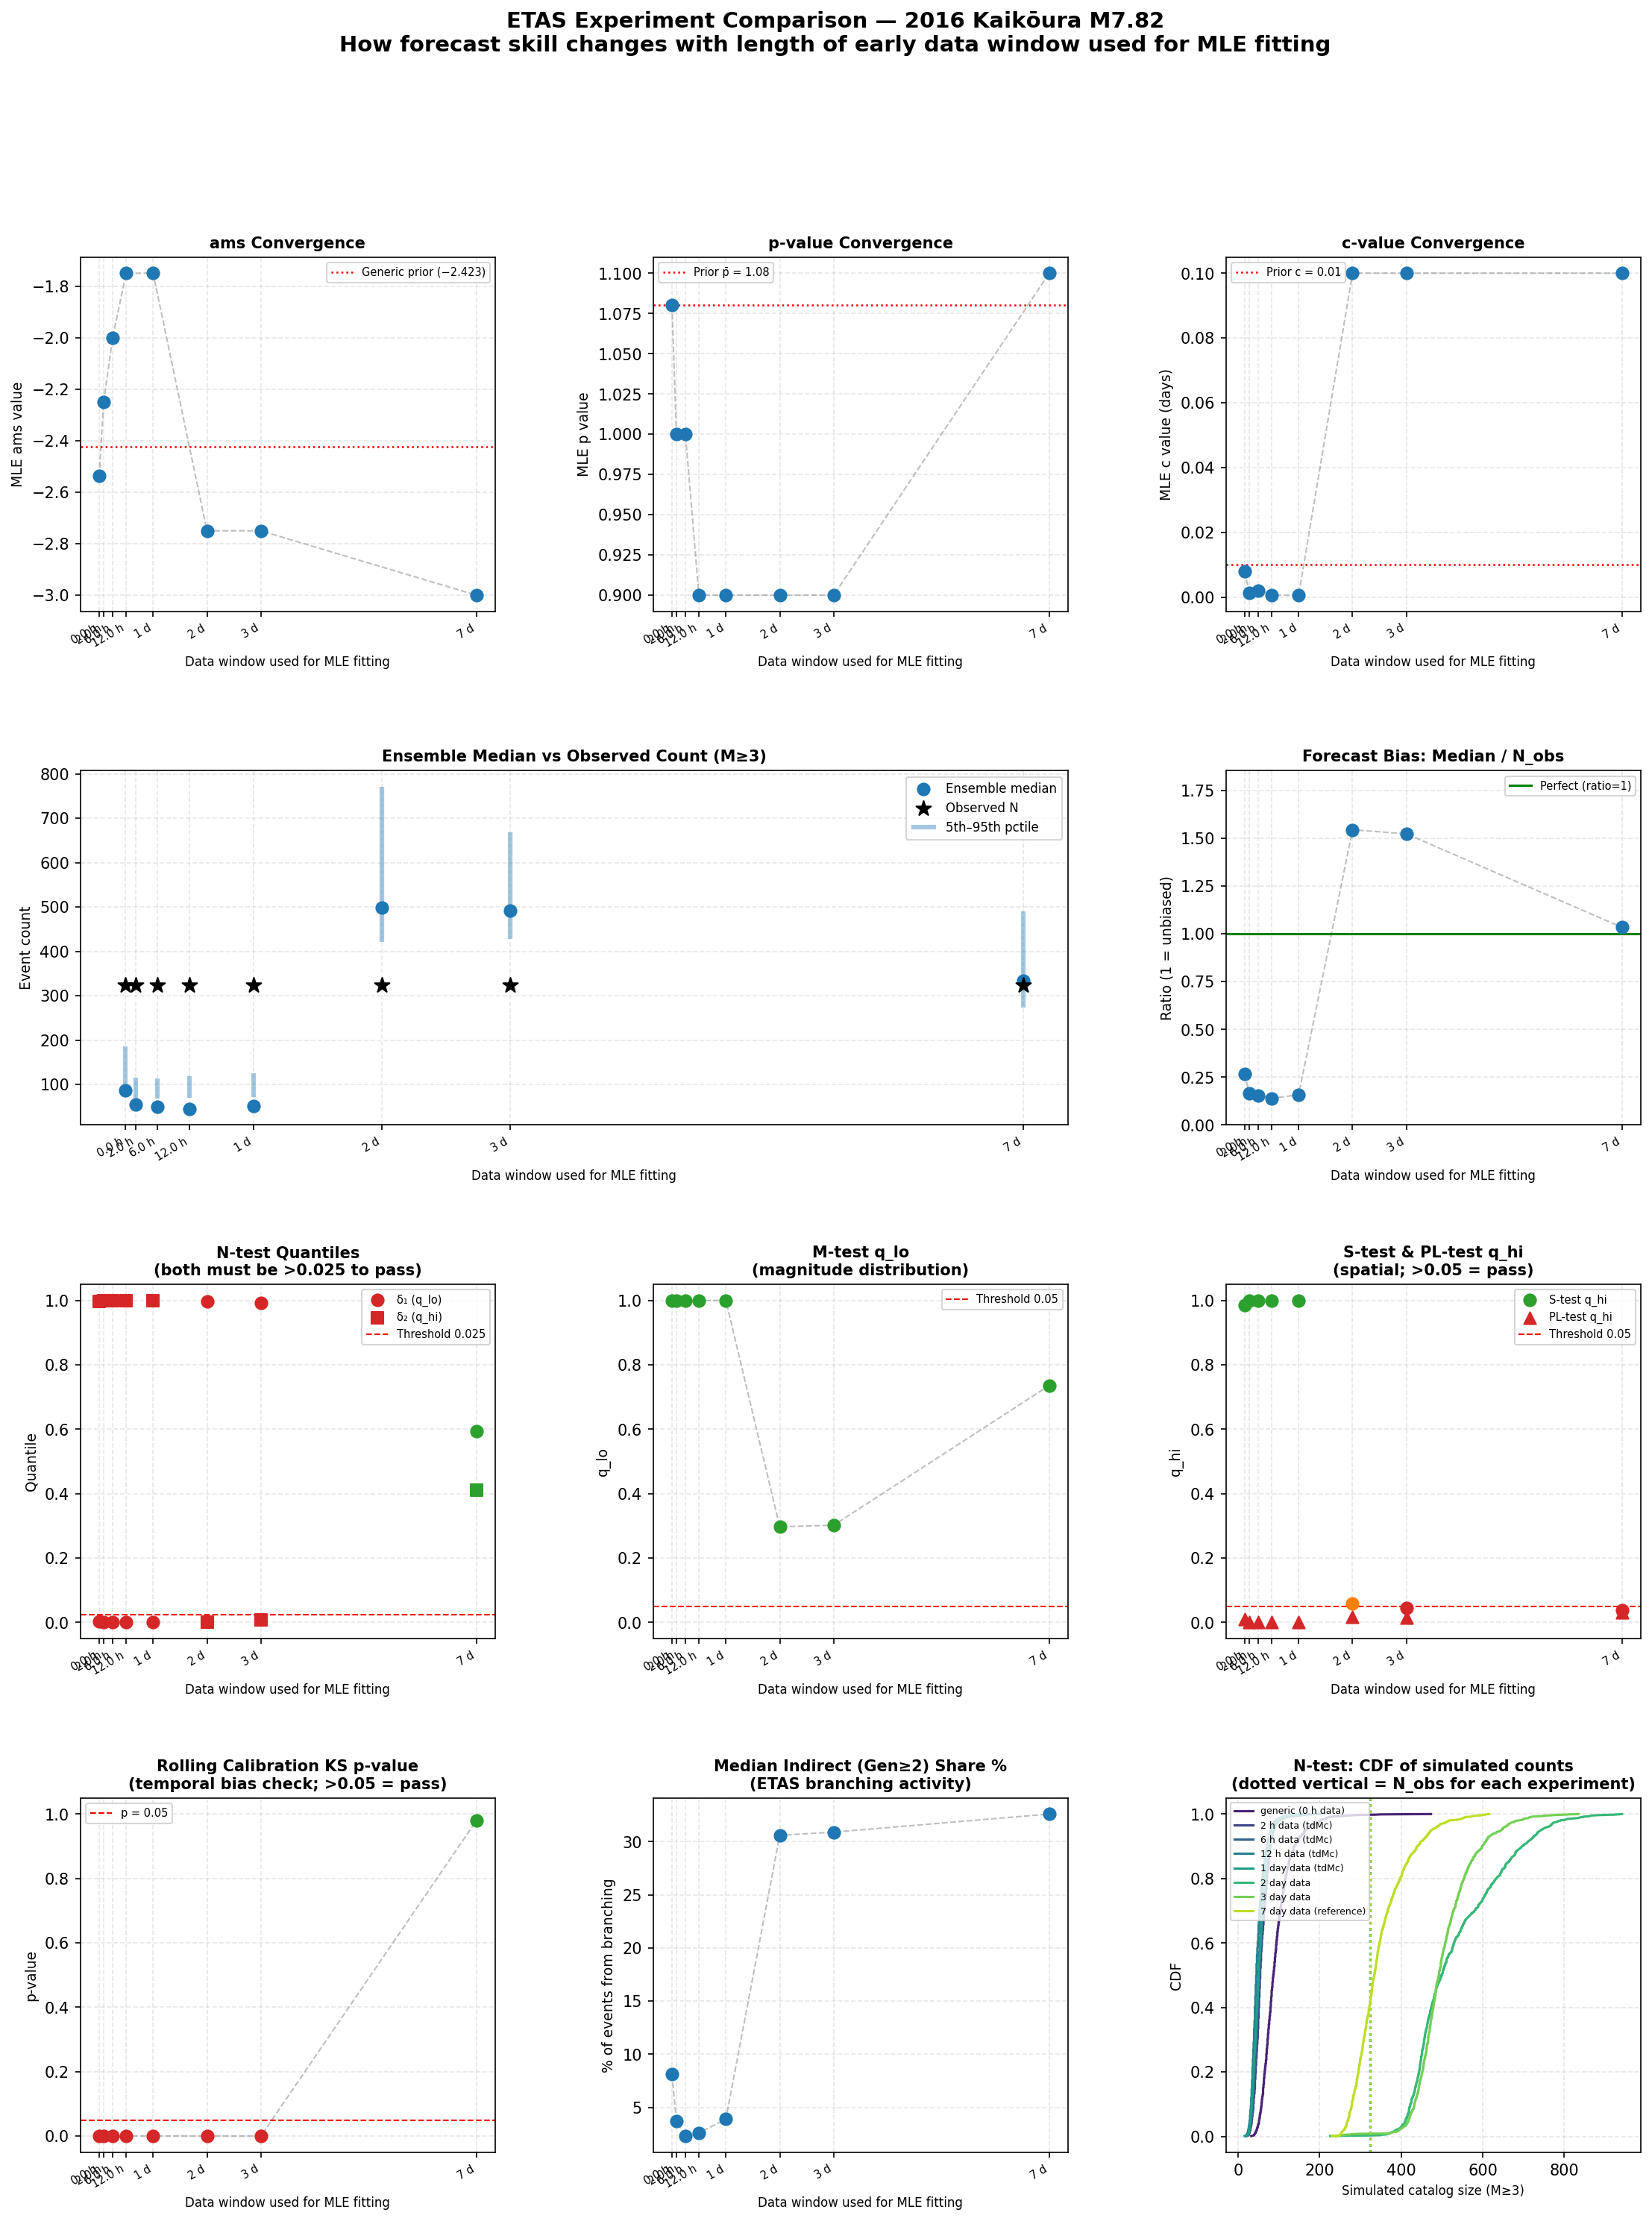
\includegraphics[width=\textwidth]{etas_experiment_comparison.png}
\caption{Multi-panel summary of the fixed-horizon issue-time experiment.
Top row: parameter evolution with issue time. Middle row: ensemble median versus
observed count ($N_{\mathrm{obs}}=323$) and the resulting count bias. Bottom
row: pyCSEP summary statistics, rolling calibration, indirect triggering share,
and empirical N-test distributions. All runs verify the same days 7--14 window;
only the fit-data window changes. The leftmost point is the generic-parameter
ETAS run conditioned on the first 0.5~d catalog. The dashed horizontal line in
the count panel marks $N_{\mathrm{obs}}=323$.}
\label{fig:comparison}
\end{figure}

\subsection{Magnitude--frequency consistency across issue times}
\label{sec:mag_freq}

A novel finding of the fixed-horizon experiment is that magnitude--frequency
skill is \emph{decoupled} from count skill: the Gutenberg--Richter distribution
is well-captured regardless of issue time.

The resampled M-test passes for all eight runs, with lower-tail quantiles of
0.744--0.852 (Table~\ref{tab:counts}). The resampled test controls for count
differences by drawing a subsample of each simulated catalog matched to the
observed count before computing the total variation distance. Its universal
passage means that the relative frequency of magnitudes among simulated events
matches the observed magnitude distribution for all issue times.

The MLL test similarly passes for all eight runs, with lower-tail quantiles of
0.324--0.390, confirming that the log-likelihood of the observed magnitudes
under the simulated ensemble is well within the central body of the simulated
distribution.

The simple (unsampled) M-test fails for the early windows (lower-tail quantile
$\approx1.000$ for 2~h--1~d). This is a count artifact: with simulation
medians of 45--51, the simulated magnitude probability mass function is
necessarily sparse and concentrated at lower magnitudes relative to the full
distribution, producing large total variation distance when compared to 323
observed events. The resampled M-test correctly identifies this as a count
confound rather than a genuine GR failure.

The operational implication is direct: the $b=1.0$ assumption underlying the NZ
ETAS implementation is robust across all issue times for this sequence. Any
operational upgrade effort should therefore prioritize count calibration
(the branching and Omori barriers described above) rather than magnitude
recalibration.

\subsection{Near-supercritical tail behavior: analytical expectation versus simulation median}
\label{sec:tails}

A critical and novel finding of this experiment is the large divergence between
the analytical expected count $E[N]$ and the pyCSEP simulation median for early
issue times:

\begin{table}[ht]
\centering
\small
\caption{Percentile distribution of simulated event counts and comparison of
analytical expected count to simulation median (days 7--14, $M\geq3$).}
\label{tab:percentiles}
\begin{tabular}{lrrrrr}
\toprule
Run & 5th pctile & Median (sim) & 95th pctile & $E[N]$ (analytical) & $E[N]$ / Median \\
\midrule
Generic & 72 & 103 & 186 & 144.9 & 1.4 \\
2 h & 66 & 85 & 115 & 252.6 & 3.0 \\
6 h & 68 & 87 & 114 & 432.2 & 5.0 \\
12 h & 69 & 87 & 119 & 921.3 & 10.6 \\
1 d & 72 & 94 & 125 & 928.7 & 9.9 \\
2 d & 421 & 513 & 771 & 403.5 & 0.79 \\
3 d & 428 & 507 & 668 & 417.5 & 0.82 \\
7 d & 273 & 341 & 490 & 265.7 & 0.78 \\
\bottomrule
\end{tabular}
\vspace{4pt}
\raggedright
\footnotesize
Median (sim) is from the simulation percentile distribution; this differs
slightly from the pyCSEP representative-catalog median used in
Table~\ref{tab:counts}. $E[N]$ is the analytical expected count from the ETAS
summary file.
\end{table}

For the 6~h run, $E[N]=432$ while the simulation median is 87, a factor of
5.0. For 12~h and 1~d, $E[N]$ is approximately 921 and 929, respectively,
while the simulation medians are 87 and 94---divergence factors of 10--11.
This is not a software error but a signature of \emph{near-supercritical ETAS
dynamics}: when the branching ratio approaches unity, the distribution of
total event counts becomes extremely right-skewed. The vast majority of
realizations produce only modest cascades (contributing to the low median), but
a small fraction of simulations produce explosive cascades that dominate the
mean and drive $E[N]$ far above the median.

For these early-window parameter sets, the branching ratio in the upper tail is
at or above the critical value of one. This means that the analytical $E[N]$,
computed from the first moment of the branching process, is not a robust
forecast summary: a single catastrophic realization can inflate it by an order
of magnitude above the typical outcome. The pyCSEP simulation \emph{median} is
the operationally safe summary because it is robust to these tail events.

The contrast with the 2~d--7~d runs is instructive: there, $E[N]$ and the
simulation median are close (ratio 0.78--0.82), consistent with a subcritical
process well below the branching instability.

\textbf{Operational warning}: for the early issue-time regime (2~h--1~d),
reporting $E[N]$ from the ETAS summary file as the forecast rate estimate would
be catastrophically misleading---producing apparent rates of 252--929 events
against a typical simulated catalog of 45--94 events. The median of the
stochastic ensemble is the only defensible operational summary statistic in
this regime.

\subsection{Spatial support diagnostics}
\label{sec:spatial}

All eight runs remain support-limited in the pyCSEP S-test and PL-test, meaning
that observed events occur in spatial cells where the forecast assigns zero
probability (Table~\ref{tab:support}). This is a persistent limitation
orthogonal to the count-calibration question.

\begin{table}[ht]
\centering
\small
\caption{Spatial support and temporal calibration diagnostics.}
\label{tab:support}
\begin{tabular}{lrrrr}
\toprule
Run & Obs.\ events in zero-rate cells & Cells affected & Zero-rate cells / 6343 & Rolling KS $p$ \\
\midrule
Generic & 25 & 18 & 2890 & $5.0\times10^{-12}$ \\
2 h (\texttt{tdMc}) & 22 & 16 & 2653 & $4.4\times10^{-18}$ \\
6 h (\texttt{tdMc}) & 17 & 13 & 2553 & $1.6\times10^{-16}$ \\
12 h (\texttt{tdMc}) & 10 & 10 & 2457 & $2.0\times10^{-21}$ \\
1 d (\texttt{tdMc}) & 11 & 11 & 2446 & $2.6\times10^{-19}$ \\
2 d & 18 & 11 & 2403 & $2.6\times10^{-5}$ \\
3 d & 16 & 14 & 2374 & $3.1\times10^{-5}$ \\
7 d & 16 & 14 & 3002 & $9.8\times10^{-1}$ \\
\bottomrule
\end{tabular}
\vspace{4pt}
\raggedright
\footnotesize
``Obs.\ events in zero-rate cells'' is the number of observed events that fall
in spatial cells where no simulated catalog placed any event. ``Cells affected''
is the number of distinct spatial cells containing at least one such observation.
\end{table}

The spatial support pattern follows the fitted kernel width: runs with fewer
data points (2~h--1~d) fit narrower spatial kernels, leaving 2446--2653 of the
6343 testing cells with zero probability mass but paradoxically producing fewer
unsupported observations (10--22) because more observed events fall within the
tighter cluster around the mainshock. Longer fitting windows (2~d--7~d) produce
broader kernels: the 7~d fit leaves only 3002 cells empty but still has 16
observed events in zero-rate locations, suggesting persistent limitation from
the isotropic kernel assumption rather than from data volume alone.

The rolling KS test is decisive in distinguishing the three regimes. Only the
7~d run passes ($p=0.98$). The 2~d and 3~d runs fail at $p\approx3\times10^{-5}$:
despite the approximately correct cumulative count, the Omori decay is too slow
in these runs and events are allocated incorrectly within the 7--14~d window.
The 2~h--1~d runs fail catastrophically ($p$ as low as $2\times10^{-21}$)
because the entire simulation count is compressed toward the beginning of the
window by near-zero $c$ values.

\section{Discussion}

\subsection{Three failure regimes as a novel observational result}

The three-regime structure identified in this analysis is only observable under
the fixed-horizon design. In any experiment where verification windows vary with
issue time, count differences reflect a mixture of issue-time effects and
horizon effects that cannot be cleanly disentangled. The uniform verification
target ($N_{\mathrm{obs}}=323$ in all cases) reveals that the transition from
underprediction to overprediction between 1~d and 2~d is a genuine property of
the MLE landscape, not an artifact of different observation windows.

The physical interpretation of the three regimes is as follows. In Regime~1
(generic and 2~h--1~d), the available data contain too few aftershock pairs for
the MLE to identify the branching structure; it converges instead to a
mainshock-dominated solution with negligible cascading. In Regime~2 (2~d--3~d),
enough aftershocks have accumulated to identify that cascading is significant
($a=-2.0$, indirect triggering $\approx31\%$), but the Omori exponent is still
underdetermined; the MLE settles on $p=0.90$ rather than the converged value of
1.10. In Regime~3 (7~d only), both the branching structure and the decay rate
are correctly identified, and the forecast is count- and temporally calibrated.

\subsection{\texttt{timeDependentMc} is necessary but not sufficient}

The \texttt{timeDependentMc} correction addresses catalog incompleteness during
fitting by down-weighting events in incomplete intervals. This is a necessary
ingredient for early ETAS forecasting, consistent with the literature
\cite{omi2013,omi2014,page2016,seif2017,hainzl2024}. However, the results here
show clearly that it is not sufficient to recover forecast skill for issue times
of 1~d or less. The 2~h--1~d runs all have \texttt{timeDependentMc=true}, yet
they all produce severely underpredictive forecasts with N-test failures at
$\delta_2=1.000$.

The reason is that the \texttt{timeDependentMc} correction addresses
\emph{which events enter the likelihood}, but it does not resolve the
identifiability problem that arises when the total number of observed events
is too small to constrain the MLE's cascade structure. Correcting for missing
events and having enough events to identify branching are separate requirements.
Real-time operational systems that apply \texttt{timeDependentMc} without also
recognizing the branching identifiability barrier will issue well-corrected but
still fundamentally underpredictive forecasts in the first day.

\subsection{Two identifiability barriers as a novel conceptual framework}

The sequence of regime transitions implies two distinct identifiability
barriers, each requiring a different amount of data:

\begin{enumerate}
    \item \textbf{The branching barrier} (crossed between 1~d and 2~d): the
    MLE requires enough aftershock-to-aftershock pairs to identify the $a$-value
    and distinguish a genuinely cascading sequence from a mainshock-dominated
    sequence. Until this barrier is crossed, the indirect triggering fraction is
    near zero and count forecasts are severely underpredictive.

    \item \textbf{The Omori barrier} (crossed between 3~d and 7~d): the MLE
    requires a sufficiently long temporal baseline to resolve the curvature of
    the Omori decay law and estimate $p$ accurately. Until this barrier is
    crossed, $p$ is underestimated and the forecast rate at days 7--14 is
    systematically too high.
\end{enumerate}

This framework suggests two targeted improvements, each addressing one barrier.
The branching barrier might be lowered by using stronger Bayesian priors on the
$a$-value or by incorporating external sequence-similarity information during
the first day. The Omori barrier is more fundamental because $p$ estimation
requires observing the temporal slope over an extended window, but it could be
addressed by a tight Bayesian prior on $p$ derived from regional or global
aftershock statistics.

\subsection{Near-supercritical behavior and the danger of reporting $E[N]$}

The divergence between $E[N]$ and simulation medians in the early-window runs
is a practically important finding. For the 12~h and 1~d parameter sets, the
analytical expectation exceeds the simulation median by factors of about 10.
This arises because the MLE solution, while not explicitly supercritical (the
branching ratio is below one in expectation), has a heavy-tailed distribution
of total offspring counts. A small fraction of simulations undergo near-critical
cascades that inflate the mean without raising the typical (median) outcome.

In operational practice, the mean $E[N]$ is the quantity most naturally
associated with the first-moment prediction of a point process, and it may be
the quantity displayed to emergency managers or communicated to the public. For
well-calibrated subcritical ETAS (as in the 7~d run), $E[N]$ and the median
are close and either is an acceptable summary. But for early issue times in
sequences like Kaik\={o}ura, reporting $E[N]$ as the ``expected'' aftershock
count could overstate the forecast by an order of magnitude relative to the
most likely outcome. Operational protocols should explicitly require reporting
the \emph{median} of the stochastic ensemble alongside any mean estimate, and
should flag large $E[N]$-to-median ratios as a near-supercritical warning.

\subsection{Bayesian priors on $p$ as the highest-leverage improvement for Regime~2}

The Regime~2 overprediction (2~d--3~d) arises specifically from $p$
underestimation. Once the branching barrier is crossed, the cascade structure
is essentially correct, and the discrepancy is concentrated in the Omori
exponent. This suggests a targeted intervention: a Bayesian prior on $p$
derived from regional or global aftershock statistics would constrain the MLE
away from the shallow-decay solution at early times without requiring additional
data.

For a sequence like Kaik\={o}ura, where regional Omori statistics might favor
$p\approx1.0$--$1.1$, a moderately informative prior could pull the 2~d and
3~d fits toward the correct $p=1.10$ value, potentially moving those runs into
or near the calibrated regime. This is a structurally different improvement
from \texttt{timeDependentMc}: it targets a different stage of the MLE problem
(parameter bounding rather than data selection) and a different failure mode
(Regime~2 rather than Regime~1).

\subsection{Relation to the literature}

These results are consistent with the early-forecast ETAS literature but add
specificity that previous studies could not provide. Omi et al.\ showed that
very early ETAS forecasting can work only when incompleteness is handled
explicitly \cite{omi2013,omi2014,omi2015}. Page et al.\ identified
time-dependent catalog incompleteness as an essential operational ingredient
\cite{page2016}, and Seif et al.\ quantified how strongly missing early events
can distort ETAS parameters \cite{seif2017}. The Kaik\={o}ura case study of
Harte likewise found that the earliest real-time ETAS forecasts were compromised
by both early catalog limitations and evolving event metadata \cite{harte2019}.

The archived NZ results fit that pattern but add two specific new observations.
First, the branching/Omori barrier distinction is more cleanly visible here than
in previous analyses because of the fixed-horizon design. Second, the
near-supercritical tail behavior and $E[N]$-versus-median divergence have not
previously been reported as a distinct operational concern for early ETAS
forecasts, to our knowledge.

The persistent spatial support limitation (16--25 observed events in zero-rate
cells across all runs) is consistent with the broader observation in aftershock
forecasting reviews \cite{hardebeck2024} that operational value depends not only
on count calibration but on spatial accuracy. Isotropic spatial kernels are a
known limitation of the basic ETAS formulation; the fact that this limitation
persists even in the well-calibrated 7~d run suggests that kernel improvements
would be complementary to, and separate from, the temporal calibration
improvements identified here.

\section{Conclusions}

The fixed-horizon issue-time experiment for the 2016 $M_w$ 7.8 Kaik\={o}ura
sequence produces the following principal conclusions.

\begin{enumerate}
    \item The fixed-horizon design (all runs verifying days 7--14,
    $N_{\mathrm{obs}}=323$) reveals \textbf{three distinct failure regimes} that
    are only separable when the verification window is held constant. Earlier
    variable-horizon analyses could not isolate these regimes.

    \item \textbf{Regime~1} (generic and 2~h--1~d): the MLE converges to a
    low-cascade local minimum (indirect triggering 2--9\%, correct value
    $\approx33\%$), producing severely underpredictive simulations
    (medians 45--103 versus $N_{\mathrm{obs}}=323$; ratios 0.14--0.32). The
    \texttt{timeDependentMc} correction is insufficient to recover forecast
    skill: the branching structure cannot be identified from hours of data,
    regardless of completeness correction.

    \item \textbf{Regime~2} (2~d--3~d): once enough data accumulate to cross
    the branching barrier (between 1~d and 2~d), the MLE correctly identifies
    the cascade structure but still underestimates the Omori exponent ($p=0.90$
    instead of 1.10). The resulting forecasts overpredict days 7--14
    (medians 492--499; ratios 1.52--1.55) and fail N-tests by overprediction.

    \item \textbf{Regime~3} (7~d only): both the branching structure and the
    Omori decay rate are correctly identified. The forecast is count-calibrated
    (median 334, ratio 1.03; N-test $(\delta_1,\delta_2)=(0.594,0.411)$) and
    temporally calibrated (rolling KS $p=0.98$).

    \item The analytical expected count $E[N]$ diverges from the simulation
    median by factors of 5--11 for the 12~h and 1~d runs, a signature of
    \textbf{near-supercritical ETAS dynamics} in the tail of the branching
    distribution. Reporting $E[N]$ as the operational forecast rate for these
    issue times would overstate the typical outcome by an order of magnitude.
    The simulation median is the only defensible operational summary statistic
    in this regime.

    \item Magnitude--frequency consistency (resampled M-test and MLL) is
    maintained \textbf{across all eight issue times}, with no significant
    deviation from the Gutenberg--Richter distribution in any run. The $b=1.0$
    assumption is robust for this sequence; operational improvement effort
    should focus on count calibration rather than magnitude recalibration.

    \item Spatial support limitations persist across all runs (16--25 observed
    events in zero-rate cells; 2374--3002 of 6343 testing cells empty), and
    are not resolved by longer fitting windows. This indicates a structural
    kernel-support limitation that is \textbf{orthogonal to} and independent of
    the temporal calibration improvements.

    \item We identify \textbf{two distinct identifiability barriers}: a
    \emph{branching barrier} (crossed near 2~d post-mainshock) and an
    \emph{Omori barrier} (crossed near 7~d). These barriers require different
    interventions: the branching barrier may be addressable with informative
    $a$-value priors or sequence-similarity methods; the Omori barrier is most
    efficiently addressed with Bayesian hierarchical priors on $p$, which
    represent the highest-leverage single improvement for the Regime~2 forecasts.
\end{enumerate}

\section*{Data and Resources}

The results summarized here were taken from the archived ETAS summary files
\texttt{nz\_etas\_simulations*.txt} and the pyCSEP output directories
\texttt{build/pycsep*} in this repository. GeoNet event metadata and observed
catalogs were accessed through the GeoNet event and catalog services during the
archived runs. pyCSEP documentation and catalog-evaluation concepts were taken
from the official documentation site \cite{pycsep_eval,pycsep_catalog_tutorial}.

\newpage
\begin{thebibliography}{99}

\bibitem{usgs_schedule}
U.S. Geological Survey (USGS), \emph{Operational Aftershock Forecast:
Automatic Forecast Update Schedule}.\\
\url{https://earthquake.usgs.gov/data/oaf/schedule.php}

\bibitem{usgs_overview}
U.S. Geological Survey (USGS), \emph{Operational Aftershock Forecast:
Overview}.\\
\url{https://earthquake.usgs.gov/data/oaf/overview.php}

\bibitem{usgs_background}
U.S. Geological Survey (USGS), \emph{Operational Aftershock Forecast:
Scientific Background}.\\
\url{https://earthquake.usgs.gov/data/oaf/background.php}

\bibitem{reasenberg1989}
P. Reasenberg and L. Jones (1989),
\emph{Earthquake hazard after a mainshock in California},
Science, 243(4895), 1173--1176.\\
\url{https://doi.org/10.1126/science.243.4895.1173}

\bibitem{ogata1988}
Y. Ogata (1988),
\emph{Statistical Models for Earthquake Occurrences and Residual Analysis for
Point Processes},
Journal of the American Statistical Association, 83(401), 9--27.\\
\url{https://doi.org/10.1080/01621459.1988.10478560}

\bibitem{ogata2006}
Y. Ogata and K. Katsura (2006),
\emph{Immediate and updated forecasting of aftershock hazard},
Geophysical Research Letters, 33, L10305.\\
\url{https://doi.org/10.1029/2006GL025888}

\bibitem{omi2013}
T. Omi, Y. Ogata, Y. Hirata, and K. Aihara (2013),
\emph{Forecasting large aftershocks within one day after the main shock},
Scientific Reports, 3, 2218.\\
\url{https://doi.org/10.1038/srep02218}

\bibitem{omi2014}
T. Omi, Y. Ogata, Y. Hirata, and K. Aihara (2014),
\emph{Estimating the ETAS model from an early aftershock sequence},
Geophysical Research Letters, 41(3), 850--857.\\
\url{https://doi.org/10.1002/2013GL058958}

\bibitem{omi2015}
T. Omi, Y. Ogata, Y. Hirata, and K. Aihara (2015),
\emph{Intermediate-term forecasting of aftershocks from an early aftershock
sequence: Bayesian and ensemble forecasting approaches},
Journal of Geophysical Research: Solid Earth, 120(4), 2561--2571.\\
\url{https://doi.org/10.1002/2014JB011456}

\bibitem{page2016}
M. T. Page, N. J. van der Elst, J. L. Hardebeck, K. R. Felzer, and
A. J. Michael (2016),
\emph{Three ingredients for improved global aftershock forecasts:
Tectonic region, time-dependent catalog incompleteness, and
intersequence variability},
Bulletin of the Seismological Society of America, 106(5), 2290--2301.\\
\url{https://doi.org/10.1785/0120160073}

\bibitem{seif2017}
S. Seif, M. T. Page, J. E. Zechar, M. E. Morgan, and J. T. McBrearty (2017),
\emph{Estimating ETAS: The effects of truncation, missing data, and model
assumptions},
Journal of Geophysical Research: Solid Earth, 122(6), 4490--4510.\\
\url{https://doi.org/10.1002/2016JB012809}

\bibitem{woessner2005}
J. Woessner and S. Wiemer (2005),
\emph{Assessing the quality of earthquake catalogues: Estimating the
magnitude of completeness and its uncertainty},
Bulletin of the Seismological Society of America, 95(2), 684--698.\\
\url{https://doi.org/10.1785/0120040007}

\bibitem{lippiello2019}
E. Lippiello, F. Petrillo, C. Godano, and L. de Arcangelis (2019),
\emph{Post Seismic Catalog Incompleteness and Aftershock Forecasting},
Geosciences, 9(8), 355.\\
\url{https://doi.org/10.3390/geosciences9080355}

\bibitem{vandere1st2021}
N. J. van der Elst (2021),
\emph{B-positive: A robust estimator of aftershock magnitude distribution in
transiently incomplete catalogs},
Journal of Geophysical Research: Solid Earth, 126(2), e2020JB021027.\\
\url{https://doi.org/10.1029/2020JB021027}

\bibitem{hainzl2024}
S. Hainzl, T. Kumazawa, and Y. Ogata (2024),
\emph{Aftershock forecasts based on incomplete earthquake catalogues:
ETASI model application to the 2023 SE T\"urkiye earthquake sequence},
Geophysical Journal International, 236(3), 1609--1619.\\
\url{https://doi.org/10.1093/gji/ggae006}

\bibitem{zhuang2011}
J. Zhuang (2011),
\emph{Next-day earthquake forecasts for the Japan region generated by the
ETAS model},
Earth, Planets and Space, 63(3), 207--216.\\
\url{https://doi.org/10.5047/eps.2010.12.010}

\bibitem{csep_etas}
Collaboratory for the Study of Earthquake Predictability (CSEP),
\emph{ETAS and ETASV1.1 models}.\\
\url{https://cseptesting.org/etas-model/}

\bibitem{rhoades2017}
D. Rhoades, M. Gerstenberger, A. Christophersen, and D. Harte (2017),
\emph{Earthquake forecasts and their applications following the M7.8 2016
Kaik\={o}ura earthquake}. Southern California Earthquake Center abstract page.\\
\url{https://central.scec.org/publication/7689}

\bibitem{harte2019}
D. Harte (2019),
\emph{Evaluation of earthquake stochastic models based on their real-time
forecasts: a case study of Kaik\={o}ura 2016},
Geophysical Journal International, 217(3), 1894--1913.\\
\url{https://doi.org/10.1093/gji/ggz088}

\bibitem{marzocchi2014}
W. Marzocchi, A. M. Lombardi, and E. Casarotti (2014),
\emph{The establishment of an operational earthquake forecasting system in
Italy},
Seismological Research Letters, 85(5), 961--969.\\
\url{https://doi.org/10.1785/0220130219}

\bibitem{spassiani2023}
I. Spassiani, G. Falcone, M. Murru, and W. Marzocchi (2023),
\emph{Operational Earthquake Forecasting in Italy: validation after 10 yr of
operativity},
Geophysical Journal International, 234(3), 2501--2518.\\
\url{https://doi.org/10.1093/gji/ggad256}

\bibitem{puertorico2022}
N. J. van der Elst, J. L. Hardebeck, A. J. Michael, S. K. McBride, and
E. Vanacore (2022),
\emph{Prospective and retrospective evaluation of the U.S. Geological Survey
public aftershock forecast for the 2019--2021 Southwest Puerto Rico
Earthquake and aftershocks},
Seismological Research Letters, 93(2A), 620--640.\\
\url{https://pubs.usgs.gov/publication/70229086}

\bibitem{hardebeck2024}
J. L. Hardebeck, A. L. Llenos, A. J. Michael, M. T. Page, M. Schneider, and
N. J. van der Elst (2024),
\emph{Aftershock forecasting},
Annual Review of Earth and Planetary Sciences, 52, 61--84.\\
\url{https://doi.org/10.1146/annurev-earth-040522-102129}

\bibitem{pycsep_eval}
pyCSEP documentation, \emph{Evaluations}.\\
\url{https://docs.cseptesting.org/concepts/evaluations.html}

\bibitem{pycsep_catalog_tutorial}
pyCSEP documentation, \emph{Catalog-based Forecast Evaluation Tutorial}.\\
\url{https://docs.cseptesting.org/tutorials/catalog_forecast_evaluation.html}

\end{thebibliography}

\end{document}
